\documentclass[a4paper, notitlepage, 10pt]{article}
\usepackage{geometry}
% WSC 2015 configs
\fontfamily{times}
\geometry{verbose,tmargin=30mm,bmargin=25mm,lmargin=25mm,rmargin=25mm}
\pagestyle{empty}
% end configs
\usepackage{setspace,relsize}               
\usepackage{moreverb}                        
\usepackage{url}
\usepackage{hyperref}
\hypersetup{colorlinks=true,citecolor=blue}
\usepackage{amsmath}
\usepackage{mathtools} 
\usepackage{amsthm}
\usepackage{amssymb}
\usepackage{indentfirst}
\usepackage{todonotes}
\usepackage[authoryear,round]{natbib}
\bibliographystyle{apalike}
\usepackage[pdftex]{lscape}
\usepackage[utf8]{inputenc}
% Title Page
\title{\vspace{-9ex}\centering \bf Choosing the weights for the logarithmic pooling of probability distributions}
\author{
Luiz Max F. de Carvalho$^{a,b,c}$, Daniel A. M. Villela$^a$, Flavio Coelho$^c$ \& Leonardo S. Bastos$^a$ \\
a -- Program for Scientific Computing (PROCC), Oswaldo Cruz Foundation. \\
b -- Institute of Evolutionary Biology, University of Edinburgh.\\
c -- School of Applied Mathematics, Getulio Vargas Foundation (FGV).
}
\DeclareMathOperator*{\argmin}{arg\,min}
\DeclareMathOperator*{\argmax}{arg\,max}
\newtheorem{theo}{Theorem}[]
\newtheorem{proposition}{Proposition}[]
\newtheorem{remark}{Remark}[]
\setcounter{theo}{0} % assign desired value to theorem counter
\begin{document}
\maketitle

\begin{abstract}
Combining different prior distributions is an important issue in decision theory and Bayesian inference.
Logarithmic pooling is a popular method to aggregate expert opinions by using a set of weights that reflect the reliability of each information source.
The resulting pooled distribution however heavily depends set of weights given to each opinion/prior.
In this paper we explore three objective approaches to assigning weights to opinions.
Two methods are stated in terms of optimisation problems and a third one uses a hierarchical prior that accounts for uncertainty on the weights. 
We explore an example in which a proportion is estimated using weights assigned to a finite set of opinions and show that, depending on the used method, results vary from discarding some of the expert opinions to the situation in which all opinions are assigned equal weights.
Nevertheless, the three methods explored in this paper lead to very similar combined priors, with very similar integrated (marginal) likelihoods.

Key-words: logarithmic pooling; expert opinion; maximum entropy; Kullback-Liebler divergence; Dirichlet prior. 
\end{abstract}

\section*{Background}

Combining probability distributions is a topic of general interest, both in the statistical~\citep{genest1986A,genest1986B} and decision theory literatures~\citep{genest1984}.
On the theoretical front, studying opinion pooling operators may give important insights on consensus belief formation and group decision making~\citep{genest1986B}.
Among the various opinion pooling operators proposed in the literature, logarithmic pooling has enjoyed much popularity, mainly due to its many desirable properties such as relative propensity consistency (RPC) and external Bayesianity (EB)~\citep{genest1986A}. 
In a practical setting, logarithmic pooling finds use in a range of fields, from infectious disease modelling~\citep{Coelho2009} and wildlife conservation~\citep{poole2000} to engineering~\citep{lind1988, savchuk1994}.

A common situation of interest is that of combining expert opinions, represented as proper probability distributions, about a quantity of interest $\theta \in \mathbf{\Theta} \subseteq \mathbb{R}^n$.
To combine these opinions using logarithmic pooling requires assigning weights to each of the experts.
These weights represent the reliability of each opinion~\citep{genest1984}.
This requirement naturally leads to the question of how to choose the weights in a meaningful fashion, according to some well-accepted optimality criterion.
There are a few proposals in the literature that build methods using different approaches.
One proposal is to maximise the entropy the pooled distribution~\citep{myung1996}, whereas another one is to minimise Kullback-Liebler (KL) divergence between the pooled distribution and the individual opinions~\citep{abbas2009} or between the pooled (prior) distribution and the posterior distribution~\citep{rufo2012A,rufo2012B}.

These approaches, while moving away from the problem of arbitrarily assigning the weights, arrive at single point solutions, similar to point estimates in Statistical theory.
Albeit acknowledging that these approaches have merit, we argue that in many settings, where one has substantial prior information on the relative reliabilities of the information sources (experts), it would be desirable to incorporate this information into the pooling procedure while accommodating uncertainty about the weights~\citep{poole2000}.
Moreover, assigning a probability distribution to the weights permits us to obtain a posterior distribution using a Bayesian procedure, which in turn enables us to learn about these weights.
Therefore, it makes possible to sequentially update knowledge about the reliability of each expert/source in the face of new data.

In this paper we explore previous approaches for deriving the weights for logarithmic pooling, namely by maximising the entropy of the resulting distribution and minimising the KL divergence between the pooled distribution and each individual distribution.
Additionally, we propose a hierarchical prior approach in which we place a Dirichlet prior on the weights.
We present an example on proportion estimation by combining Beta priors.

In what follows, we introduce the necessary theory and extend a previous 
result~\citep{poole2000} for combining more than two distributions.

Let $\mathbf{F(\theta)} = \{f_0(\theta), f_1(\theta), f_2(\theta), \ldots, f_K(\theta)\}$ be the set of prior distributions representing the opinions of $K+1$ experts and let $\boldsymbol\alpha =\{\alpha_0, \alpha_1, \alpha_2, \ldots, \alpha_K \}$ be the vector of weights, such that $\alpha_i > 0\: \forall i$ and $\sum_{i=0}^K \alpha_i = 1$.
Then the log-pooled prior is
\begin{equation}
\label{eq:logpool}
 \pi(\theta) = t(\boldsymbol\alpha) \prod_{i=0}^K f_i(\theta)^{\alpha_i} 
\end{equation}
where $t(\boldsymbol\alpha) = \int_{\boldsymbol\Theta}\prod_{i=0}^K f_i(\theta)^{\alpha_i}d\theta$.

Logarithmic pooling will only yield proper probability distributions if it is possible to normalise the expression in (\ref{eq:logpool}).
This condition is usually assumed implicitly, without proof.
\citet{poole2000} provide a proof for the case of two densities (see Theorem 1 therein), which we extend for the case of a finite number of densities.
\begin{theo}
\label{thm:normalisation}
Let $A$ be the $(K+1)$-dimensional open simplex on $[0,1]$.
For all $\boldsymbol\alpha \in A$ there exists a constant $t(\boldsymbol\alpha)$ such that $\int_{\boldsymbol\Theta}\pi(\theta)d\theta = 1$.
\end{theo}

Here we provide a simple proof using H\"{o}lder's inequality.
\begin{proof}
We begin by noting that $\pi(\theta)$ can be re-written as:
\begin{equation}
\label{eq:pirewritten}
 \pi(\theta) \propto f_0(\theta)\prod_{j=1}^{K} \left(\frac{f_j(\theta)}{f_0(\theta)}\right)^{\alpha_j}
\end{equation}
Let $X_j = \frac{f_j(\theta)}{f_0(\theta)}, j=1, 2,\ldots, K$. 
Then integrating the expression in (\ref{eq:pirewritten}) is equivalent to finding 
\begin{equation}
\label{eq:expectations}
E_{0}\left[\prod_{j=1}^KX_j^{\alpha_j}\right] \leq \prod_{j=1}^KE_{0}[X_j]^{\alpha_j}
\end{equation}
where $E_{0}[\cdot]$ is the expectation w.r.t $f_0$ and (\ref{eq:expectations}) follows from H\"{o}lder's inequality for expectations~\citep{yeh2011}.
Since we have, $\forall j$, $ E_{0}[X_j]^{\alpha_j} = \left(\int_{\boldsymbol\Theta}f_0(\theta)\frac{f_j(\theta)}{f_0(\theta)}\right)^{\alpha_j}d\theta=1^{\alpha_j}=1$, Theorem~\ref{thm:normalisation} is proven.
\end{proof}

We now move on to study three approaches to assign weights, the first two approaches based on optimality criteria and a proposal based on pooling Dirichlet prior distributions.

\section*{Choosing the weights based on optimality criteria}
\subsection*{Maximum entropy}

In a context of near complete uncertainty about the relative reliabilities of the experts (information sources) it may be desirable to combine the prior distributions such that $\pi(\theta)$ is maximally uninformative.
Such approach would ensure that, given the constraints imposed by $\mathbf{F(\theta)}$, the pooled distribution is the one which best represents the current state of knowledge~\citep{jaynes1957,savchuk1994}.
In order to choose $\boldsymbol\alpha$ so as to maximise prior 
diffuseness, one can maximise the entropy of the log-pooled prior:
\begin{equation}
\label{eq:entropypiA}
H_{\pi}(\theta) = E_{\pi}\left[-\ln\pi(\theta) \right] =-\int_{\boldsymbol\Theta}\pi(\theta)\ln\pi(\theta)d\theta 
\end{equation}

In some cases it may be useful to express $H_{\pi}(\theta)$ as
\begin{equation}
\label{eq:entropypiB}
 H_{\pi}(\theta; \boldsymbol\alpha) = \sum_{i=0}^{K} \alpha_i E_{\pi}[ - \ln f_i(\theta)] - \ln t(\boldsymbol\alpha)
\end{equation}
Formally, we want to find $\hat{\boldsymbol\alpha}$ such that
\begin{equation}
\label{eq:argmaxEnt}
 \hat{\boldsymbol\alpha}:= \argmax H_{\pi}(\theta; \boldsymbol\alpha)  
\end{equation}

This approach, however, does not result in a convex optimisation problem, therefore one is not guaranteed to find a unique solution. 
See Proposition~\ref{prop:uniqueness}, below, for intuition as to why.

\subsection*{Minimising Kullback-Liebler divergence}

One could also want to choose the pooling weights so as to minimise the total Kullback-Liebler divergence between each proposed distribution and the pooled distribution.
Let $d_i = \text{KL}(f_i || \pi)$ and let $L(\boldsymbol\alpha)$ be a loss function such that
\begin{align}
L(\boldsymbol\alpha) &= \sum_{i=0}^Kd_i \\
\label{eq:KLexpanded}
     &= -K\ln t(\boldsymbol\alpha) + \sum_{i=0}^K\sum_{j\neq i}^K\alpha_j\text{KL}(f_i||f_j) \\
     \label{eq:argminKL}
     \hat{\boldsymbol\alpha}:=& \argmin L(\boldsymbol\alpha)   
\end{align}

\begin{proposition}
\label{prop:uniqueness}
 The distribution obtained following~(\ref{eq:argminKL}) is unique, i.e., there is only one aggregated prior $\pi(\theta)$ that minimizes $L(\boldsymbol\alpha)$.
\end{proposition}
This property is proven in~\cite{rufo2012A}.
One can get some intuition into the proof  of this claim by noting that minimising~(\ref{eq:KLexpanded}) is equivalent to maximising $\ln t(\boldsymbol\alpha) = \ln\int_{\boldsymbol\Theta}\prod_{i=0}^{K}f_i(\theta)^{\alpha_i}d\theta$. 
\cite{rufo2012A} show that $t(\boldsymbol\alpha)$ is concave, therefore the problem in~(\ref{eq:argminKL}) has a unique solution.
By contrast, the problem in~(\ref{eq:argmaxEnt}) requires to minimise $\ln t(\boldsymbol\alpha)$ hence lacking a sufficient condition for the existence of a unique solution.

\section*{Specifying a prior distribution for $\boldsymbol\alpha$}

In this section we propose a hierarchical prior for $\theta$ conditional on $\boldsymbol\alpha$ in order to incorporate uncertainty on the weights.
A natural choice for a prior distribution for $\boldsymbol\alpha$ is the $(K+1)-$dimensional Dirichlet distribution.
The conditional distribution $\pi(\theta|\boldsymbol\alpha)$ is of the form in~(\ref{eq:logpool}) and the prior density for $\boldsymbol\alpha$ is 
\begin{equation}
 \label{eq:generalcondprior}
 \pi(\boldsymbol\alpha) = \frac{1}{\mathcal{B}(\boldsymbol X)}\prod_{i=0}^K \alpha_i^{x_i-1}
\end{equation}
where $\boldsymbol X = \{ x_0, x_1, \ldots, x_K\}$ is the vector of hyperparameters for the Dirichlet prior and $\mathcal{B}(X)$ is the multinomial beta function.
The marginal prior for $\theta$ is then
\begin{align}
 \label{eq:marginalhierprior}
 \pi(\theta) &= \int_{A}\pi(\theta|\boldsymbol\alpha)\pi(\boldsymbol\alpha)d\boldsymbol\alpha \\
             &= \frac{1}{\mathcal{B}(\boldsymbol X)}\int_{A}t(\boldsymbol\alpha)\prod_{i=0}^K f_i(\theta)^{\alpha_i}\alpha_i^{x_i-1}d\boldsymbol\alpha 
\end{align}

\section*{Application: binomial probabilities}

We now turn our attention to combining expert opinions about probabilities and proportions.
In this setting we are interested in the random variable $Y\sim Bernoulli(\theta)$.
Again let us assume that we want to obtain a combined prior for a proportion $\theta$.
A common choice for $\mathbf{F}(\theta)$ is the Beta family of distributions:
$$f_i(\theta;a_i, b_i) = \frac{\Gamma(a_i + b_i)}{\Gamma(a_i b_i)} \theta^{a_i-1}(1-\theta)^{b_i-1}$$
The log-pooled prior is then
\begin{align}
\pi(\theta)&=\prod_{i=0}^{K}f_i(\theta;a_i,b_i)^{\alpha_i}\\
&\propto \prod_{i=0}^{K} \left(\theta^{a_i-1}(1-\theta)^{b_i-1} \right)^{\alpha_i}\\
\label{eq:betabern}
&\propto \theta^{a^*-1}(1-\theta)^{b^*-1}
\end{align}
with $a^* =\sum_{i=0}^{K}\alpha_ia_i$ and $b^* = \sum_{i=0}^{K}\alpha_ib_i$.
Again, (\ref{eq:betabern}) is the kernel of a Beta distribution with parameters $a^*$ and $b^*$, thus 
\begin{equation}
 \label{eq:entropybeta}
 H_{\pi}(\theta) = \ln B(a^*,b^*) - (a^*-1)\psi(a^*) - (b^*-1)\psi(b^*) + (a^*+b^* -2)\psi(a^*+b^*)
\end{equation}

For the beta family of distributions, the KL divergence between $f_i(\theta)$ and $\pi(\theta)$ is
\begin{equation}
\begin{split}
 \label{eq:KLbeta}
 d_i = KL(f_i||\pi) = \ln\left(\frac{\mathcal{B}(a^*, b^*)}{\mathcal{B}(a_i, 
b_i)}\right) &+ (a_i-a^*)\psi(a_i)+ (b_i-b^*)\psi(b_i) \\
 &+ (a^*-a_i + b^* - b_i)\psi(a_i+b_i)
\end{split}
 \end{equation}

The marginal prior for $\theta$ is
\begin{equation}
\label{eq:marginalbeta}
\pi(\theta) = \frac{1}{\mathcal{B}(X)}\int_{A} \frac{1}{\mathcal{B}(a^*, b^*)} \theta^{a^* -1}(1-\theta)^{b^* -1}\alpha_i^{x_i-1}d\boldsymbol\alpha 
\end{equation}
which can also be efficiently approximated through Monte Carlo sampling.
We provide a simple implementation using the Stan~\citep{stan2014} probabilistic programming language at~\url{https://github.com/maxbiostat/opinion_pooling}.
R code for the methods, figures and tables presented in this paper can also be found at the above link.

Here we analyse an example proposed by~\cite{savchuk1994} (also discussed in~\cite{rufo2012B}) in which four experts are required supply prior information about the survival probability of a certain unit for which there have been $y = 9$ successes out of $n = 10$ trials.
The experts express their opinion as prior means for the survival probability, which~\cite{savchuk1994} then use to construct prior distributions with maximum variance given the restriction on the means.
From the vector of prior means $\mathbf{m} = \{ m_0 = 0.95, m_1 = 0.80, m_2 = 0.90, m_3 = 0.70 \}$, the authors obtain the parameters of the beta distributions for each expert,  $\mathbf{a} = \{ a_0 = 18.10, a_1 = 3.44 , a_2 = 8.32, a_3 = 1.98 \}$ and  $\mathbf{b} = \{ b_0 = 0.955 , b_1 = 0.860, b_2 = 0.924, b_3 = 0.848\}$.
The resulting prior densities are show in the top panel of Figure~\ref{fig:priors_posteriors_beta}.
To complete the analysis, we place a diffuse $Dirichlet(\boldsymbol\alpha | \boldsymbol X)$ prior on $\boldsymbol\alpha$ with $X_i = 1/4 \: \forall i$.
Finally, we propose to compare the prior distributions representing the experts' opinions as well as the combined distributions obtained by the different approaches using the integrated (marginal) likelihood (\cite{raftery2007}, eq. 9), $l(y) = \int_{0}^{1}f(\theta|y)\pi(\theta)d\theta$.
\begin{align}
 \label{eq:marglike}
 l(y_i) &= \int_{0}^{1}f(\theta|y_i, n_i)\pi(\theta)d\theta\nonumber\\
      &= \prod_{i}\frac{\Gamma(n_i-1)}{\Gamma(n_i-y_i + 1)\Gamma(y_i+1)}\frac{\Gamma(a +b)}{\Gamma(a +b + n_i)}\frac{\Gamma(a + y_i)}{\Gamma(a)}\frac{\Gamma(b + n_i - y_i) }{\Gamma(b)}
\end{align}
\section*{Results and avenues of future research}

Table~\ref{tab:alphasBeta} lists the weights proposed by each method.
Figure~\ref{fig:priors_posteriors_beta} shows the prior and posterior distributions in each of the methods and also the case in which we assign an equal weight ($1/K$) to each opinion.
It is interesting to note that maximum entropy suggests to discard all opinions but one, which effectively leads to the maximum entropy.
Since $t(\boldsymbol\alpha)$ is concave, we expect to find the maximum entropy given by the boundary conditions, which may lead to border points in the simplex.
Minimising Kullback-Liebler divergence between each prior and the pooled prior leads to finding a unique solution but in this case also suggests to discard two of the opinions.
By contrast, using a hierarchical Dirichlet prior for the weights gives rather different results from the first two methods in proposing almost equal weights to each of the opinions.
One can get insight into these results by looking at the integrated likelihoods in Table~\ref{tab:marglikes} and the densities in Figure~\ref{fig:priors_posteriors_beta}, we note that all three methods lead  to similar pooled distributions.
Note that the only distribution with a substantially different $l(y)$ is that of Expert 3, who gave a rather divergent mean for the survival probability ($m_3=0.70$).

In conclusion, if the prior distributions (opinions) are not radically different, all three methods will probably lead to similar combined priors.
Although this is the case for the simple univariate example presented, it remains to be seen if this is the case for high-dimensional $\theta$ under complex sampling distributions.
As the results presented in this paper make clear, future research shall be focused on cases where there is substantial heterogeinity in the available opinions.
Moreover, a sensitivity analysis for $\pi(\boldsymbol\alpha)$ is desirable to understand how much we can lead about the experts reliabilities~\textit{a posteriori}.

\begin{table}[ht]
\caption{Weights obtained using the three methods for the proportion estimation problem. $^1$ -- Kullback-Liebler $^2$ -- Posterior mean for $\boldsymbol\alpha$.}
\centering
\begin{tabular}{ccccc}
  \hline
Method  & $\alpha_0$ & $\alpha_1$ & $\alpha_2$ & $\alpha_3$ \\ 
  \hline
Maximum entropy & 0.00 & 1.00 & 0.00 & 0.00 \\ 
Minimum KL$^1$ divergence& 0.04 & 0.96 & 0.00 & 0.00 \\ 
Hierarchical prior$^2$ & 0.26 & 0.24 & 0.26 & 0.23 \\ 
   \hline
\end{tabular}
\label{tab:alphasBeta}
\end{table}

\begin{table}[ht]
\caption{Integrated likelihoods ($l(y)$) for the priors of each expert as well as the combined priors.
$^1$ Calculated using the posterior mean of $\boldsymbol\alpha$}
\centering
\begin{tabular}{cccc}
   \hline
   \multicolumn{2}{c}{Expert priors} &  \multicolumn{2}{c}{Pooled priors} \\
   \hline
   Expert 0 & 0.237 & Equal weights & 0.254\\
   Expert 1 & 0.211 & Maximum entropy & 0.211 \\
   Expert 2 & 0.256 & Minimum KL & 0.223\\ 
   Expert 3 & 0.163 & Hierarchical$^1$ & 0.255 \\
   \hline
\end{tabular}
\label{tab:marglikes}
\end{table}
%%%%%%%%%%%%%%%%%%%%
%\begin{table}[ht]
%\centering
%\begin{tabular}{ccc}
%  \hline
%Method & Prior & Posterior  \\ 
%  \hline
%  Equal weights & 0.90 (0.64--1.00) & 0.90 (0.73--0.99) \\ 
%  Maximum entropy & 0.80 (0.37--1.00) & 0.87 (0.66--0.98) \\ 
%  Minimum KL  & 0.82 (0.42--1.00) & 0.87 (0.67--0.99) \\ 
%  Hierarchical prior & 0.88 (0.53--1.00) & 0.90 (0.71--0.99) \\ 
%   \hline
%\end{tabular}
%\label{tab:prior_posteriorsBeta}
%\end{table}
%%%%%%%%%%%%%%%%%%%%
\section*{Acknowledgements}
The authors would like to thank Professor Adrian Raftery (University of Washington) for helpful suggestions.
DAMV was supported in part by Capes under Capes/Cofecub project (N. 833/15).
FCC is grateful to Funda\c{c}\~ao Getulio Vargas for funding during this 
project.
% {\footnotesize
\bibliography{WSC2015}
% }

\begin{figure}[!ht]
\centering
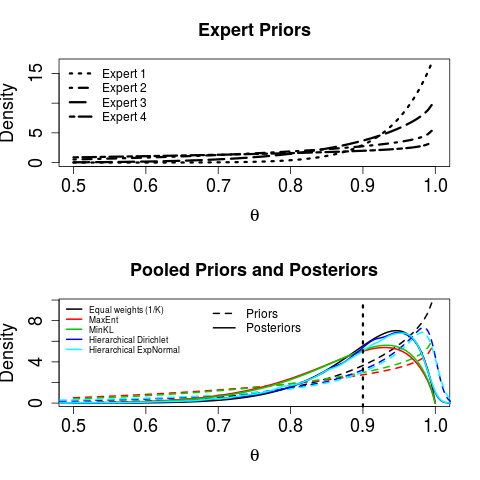
\includegraphics[width=\textwidth, height = 15cm]{figures/new_beta_example.png}
\caption{\textbf{Prior and posterior densities for $\theta$}.
Top panel shows the distributions elicited by each expert (data from~\cite{savchuk1994}) and the bottom panel shows the pooled priors and posteriors obtained using each of the three methods discussed in this paper.
The dashed vertical line marks the maximum likelihood estimate of $\theta$, $\hat{\theta}= 9/10$.}
\label{fig:priors_posteriors_beta}
\end{figure}
\end{document}          
